\documentclass[11pt]{article}
\usepackage{goldsteinnotes}
\usepackage{cancel}
\usepackage{fancybox}

\graphicspath{{figures/}}

\newcommand{\Om}{\Omega}
\newcommand{\half}[1]{\tfrac{#1}{2}}

\title{Scattering by a Central Potential;\\ the Hamiltonian}
\author{HC 6001 \quad--\quad Dr.\ Castillo}
\date{22 October 2024}

\begin{document}
\maketitle

\section*{Scattering by a central potential}

\begin{align*}
\text{Incident energy}    &: & E   &= \frac{m}{2}\,v_0^{2}, \\
\text{Incident velocity}  &: & v_0 &= \sqrt{2E/m}, \\
\text{Angular momentum}   &: & \ell &= s\,m\,v_0 = s\sqrt{2mE},
  & s &= \frac{\ell}{\sqrt{2mE}}.
\end{align*}

\[
\d^{3}r = r^{2}\,\d r\,\underbrace{\d\varphi\,\sin\theta\,\d\theta}_{\d\Om},
\qquad
\text{scattered ring solid angle:}\quad \d\Om = 2\pi\sin\theta\,\d\theta .
\]

The azimuthal angle $\varphi$ is irrelevant by symmetry, so the deflection is
controlled by $s(\theta,E)$: the impact parameter and the scattering angle are in
one-to-one correspondence, $s \longleftrightarrow \theta$.

\begin{figure}[htbp]
\centering
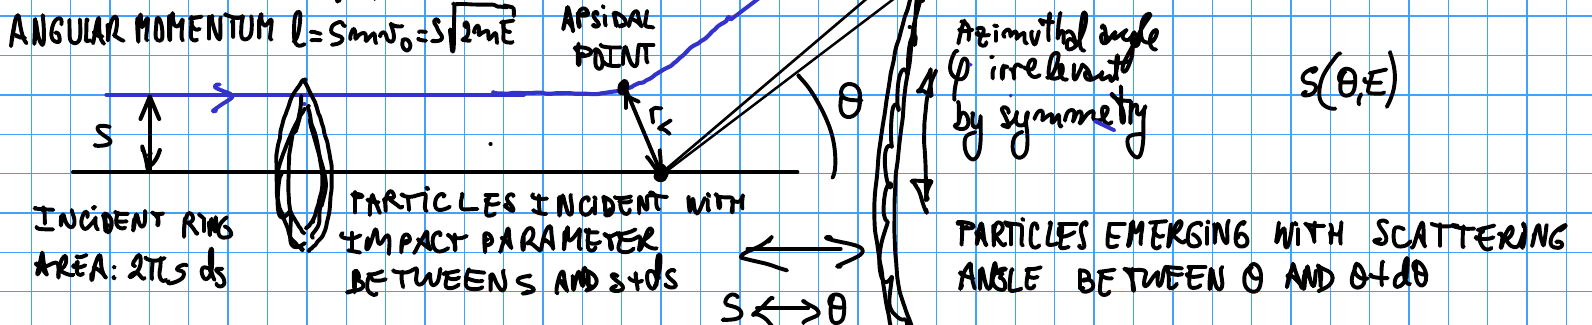
\includegraphics[width=\textwidth]{scat_fig1_beam_ring.png}
\caption{Particles incident in the ring of area $2\pi s\,\d s$ emerge into the ring
of scattering angles between $\theta$ and $\theta+\d\theta$; $r_{<}$ is the distance
of closest approach, reached at the apsidal point.}
\label{fig:beamring}
\end{figure}

\subsection*{Incident intensity; differential cross section}

\[
I = \frac{\#\ \text{particles incident per unit time}}{\text{incident beam cross-section area}},
\]
\[
\sigma(\Om)\,\d\Om
 = \frac{\#\ \text{particles scattered into }\d\Om\text{ per unit time}}{\text{incident intensity}} .
\]

\begin{align*}
I\,(2\pi s)\,\lvert \d s\rvert
  &= \#\ \text{particles going through the ring between } s \text{ and } s+\d s\\
  &= \#\ \text{particles emerging with angle between } \theta \text{ and } \theta+\d\theta\\
  &= I\,\sigma(\theta)\,2\pi\sin\theta\,\lvert \d\theta\rvert .
\end{align*}

Therefore
\[
\boxeq{\ \sigma(\theta) = \frac{s}{\sin\theta}\left\lvert \dd{s}{\theta}\right\rvert\ }
\qquad\qquad
\text{define also the total cross section:}\quad
\boxeq{\ \sigma_{T} = \int \d\Om\ \sigma(\Om)\ }
\]

\subsection*{Repulsive and attractive geometry}

\begin{figure}[htbp]
\centering
\begin{minipage}[b]{0.40\textwidth}
  \centering
  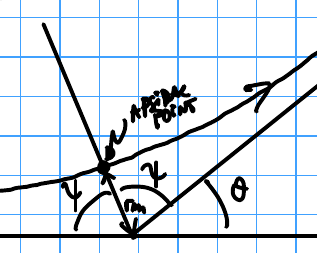
\includegraphics[width=\linewidth]{scat_fig2_repulsive.png}\\[2pt]
  {\small Repulsive case}
\end{minipage}\hfill
\begin{minipage}[b]{0.55\textwidth}
  \centering
  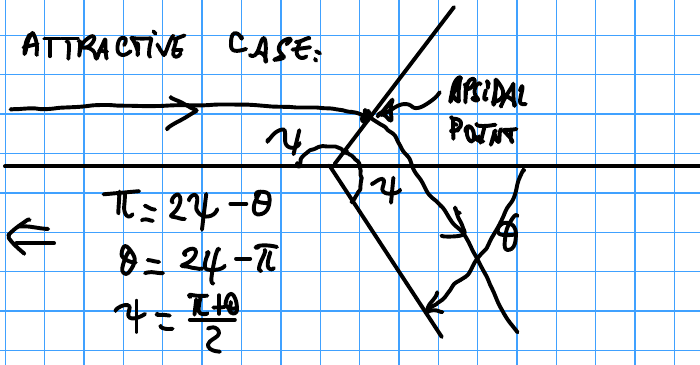
\includegraphics[width=\linewidth]{scat_fig3_attractive.png}\\[2pt]
  {\small Attractive case}
\end{minipage}
\caption{The apsidal angle $\psi$ and the scattering angle $\theta$ in the two cases.}
\label{fig:cases}
\end{figure}

\begin{center}
\begin{tabular}{@{}l@{\qquad}l@{}}
\textsc{Repulsive case} & \textsc{Attractive case}\\[4pt]
$\pi = \theta + 2\psi$ & $\pi = 2\psi - \theta$\\[2pt]
$\theta = \pi - 2\psi$ & $\theta = 2\psi - \pi$\\[2pt]
$\psi = \dfrac{\pi-\theta}{2}$ & $\psi = \dfrac{\pi+\theta}{2}$
\end{tabular}
\end{center}

In all cases:
\[
\boxeq{\ \theta = \lvert\, \pi - 2\psi\, \rvert\ }
\]

\subsection*{Computing \texorpdfstring{$s(\theta,E)$}{s(theta,E)} (universal method)}

\[
E = \frac{m}{2}\,\dot r^{2} + V(r) + \frac{\ell^{2}}{2mr^{2}},
\qquad
\dot r = \left[\frac{2}{m}\left(E - V(r) - \frac{\ell^{2}}{2mr^{2}}\right)\right]^{1/2},
\qquad
\dot r = \dd{r}{t} \;\Rightarrow\; \d t = \frac{\d r}{\dot r}.
\]

\begin{align*}
\ell = m r^{2}\dot\theta \;\Rightarrow\;
\dd{\theta}{t} = \dot\theta = \frac{\ell}{mr^{2}}
\;\Rightarrow\;
\d\theta &= \dot\theta\,\d t = \frac{\ell}{mr^{2}}\,\d t
 = \frac{\ell}{mr^{2}}\,
   \frac{\d r}{\left[\frac{2}{m}\left(E-V(r)-\frac{\ell^{2}}{2mr^{2}}\right)\right]^{1/2}}\\[4pt]
 &= \underbrace{\frac{\ell}{m}\sqrt{\frac{m}{2E}}}_{\;=\;\frac{\ell}{\sqrt{2mE}}\;=\;s}\;
    \frac{r^{-2}\,\d r}{\left[1 - \dfrac{V(r)}{E}
      - \underbrace{\dfrac{\ell^{2}}{2mE}}_{\;=\;s^{2}}\dfrac{1}{r^{2}}\right]^{1/2}} .
\end{align*}

Integrating from the apsidal point out to infinity gives the apsidal angle
$\psi$;\footnote{As written in the source, the integrand of the $r$-integral below
carries $V(r)$ rather than $V(r)/E$: the division by $E$ is omitted here although
the boxed result on the same line does carry $V(1/u)/E$. Reproduced as written.}
the substitution $u = 1/r$ is then made.\footnote{The substitution is written in the
source as $u = 1/r$, $\d u = r^{-2}\,\d r$; the correct relation is
$\d u = -r^{-2}\,\d r$. The missing sign is absorbed by the interchange of the
limits of integration. Reproduced as written.}

\begin{gather*}
\psi = \int_{0}^{\psi}\d\psi = \int_{\theta_{m}}^{\pi}\d\theta
     = \int_{r_{m}}^{\infty} \frac{s\,r^{-2}\,\d r}
       {\bigl[1 - V(r) - s^{2}/r^{2}\bigr]^{1/2}}\,,
\qquad
u = \frac{1}{r},\quad \d u = r^{-2}\,\d r,\quad u_{m} = \frac{1}{r_{m}}\\[6pt]
\Longrightarrow\quad
\boxeq{\ \theta(s) = \left\lvert\, \pi - 2\int_{0}^{u_{m}}
  \frac{s\,\d u}{\left[1 - \dfrac{V(1/u)}{E} - s^{2}u^{2}\right]^{1/2}} \,\right\rvert\ }
\end{gather*}

From here, compute
\[
\left\lvert \dd{s}{\theta}\right\rvert = \frac{1}{\left\lvert \dd{\theta}{s}\right\rvert}
\qquad\text{and use it to get}\qquad
\sigma(\theta) = \frac{s}{\sin\theta}\left\lvert \dd{s}{\theta}\right\rvert .
\]

\begin{caveat}
Up to here, results are valid for \underline{any} central potential $V(r)$.
\end{caveat}

\section*{Coulomb scattering}

\[
\text{Force}\qquad
f = \frac{Z Z' e^{2}}{r^{2}}\,,
\qquad
\raisebox{-0.42\height}{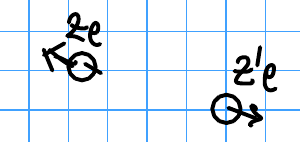
\includegraphics[width=0.15\textwidth]{scat_fig0_charges.png}}
\qquad
f = -\frac{k}{r^{2}}\,,\quad V = -\frac{k}{r}\,,
\]
\[
k = -Z Z' e^{2}.
\]

\begin{center}
\fbox{\begin{minipage}{0.52\textwidth}
\begin{tabular}{@{}ll@{}}
$E > 0$ & hyperbolic\\
$E = 0$ & parabolic\\
$E < 0$ & elliptic
\end{tabular}\\[4pt]
Only for $V = -\dfrac{k}{r}$ !!!
\end{minipage}}
\end{center}

\subsection*{Scattering: \texorpdfstring{$E>0$}{E>0}}

\[
\frac{1}{r} = C\bigl[\,1 + \varepsilon\cos(\tilde\theta - \tilde\theta\,')\,\bigr],
\qquad
C = \frac{mk}{\ell^{2}} = -\frac{m}{\ell^{2}}\,Z Z' e^{2}.
\]

\begin{gather*}
\text{Eccentricity}\quad
\varepsilon = \left[1 + \frac{2E\ell^{2}}{m k^{2}}\right]^{1/2}
 = \left[1 + \frac{2E\ell^{2}}{m\,(Z Z' e^{2})^{2}}\right]^{1/2}
 = \left[1 + \left(\frac{2sE}{Z Z' e^{2}}\right)^{2}\right]^{1/2} > 1,\\[4pt]
\ell = s\,m\,v_{0} = s\sqrt{2mE}
 \;\longrightarrow\;
 \frac{2\ell^{2}E}{m} = \frac{s^{2}\,2^{2}\,\cancel{m}\,E^{2}}{\cancel{m}}
 = (2sE)^{2}.
\end{gather*}

Two situations:
\begin{enumerate}[label=\roman*)]
\item Repulsive case \quad $Z Z' > 0 \;\Rightarrow\; k = -Z Z' e^{2} < 0$;
\item Attractive case \quad $Z Z' < 0 \;\Rightarrow\; k = -Z Z' e^{2} > 0$
      \quad (also gravity, $k = G m_{1} m_{2}$).
\end{enumerate}

\subsection*{i) Repulsive case: \texorpdfstring{$k<0$}{k<0}, \texorpdfstring{$C = mk/\ell^2 < 0$}{C = mk/l2 < 0}}

\begin{align*}
\frac{1}{r} = C\bigl[1 + \varepsilon\cos(\tilde\theta-\tilde\theta\,')\bigr] > 0
&\iff 1 + \varepsilon\cos(\tilde\theta-\tilde\theta\,') < 0\\
&\iff \varepsilon\cos(\tilde\theta-\tilde\theta\,') < -1
 \iff \cos(\tilde\theta-\tilde\theta\,') < -\frac{1}{\varepsilon}.
\end{align*}

We need the cosine to be \underline{negative} and larger in magnitude than
$1/\varepsilon$. In this case, $\tilde\theta = \tilde\theta\,'$ is not a physical
point, because
\[
\cos(\tilde\theta\,'-\tilde\theta\,') = \cos(0) = 1
\;\Longrightarrow\;
\underbrace{\frac{1}{r} = C\,[1+\varepsilon] < 0}_{\textsc{unphysical}}\,.
\]

So $\tilde\theta = \tilde\theta\,'$ is in the middle of the inaccessible region
\retracted{of} the hyperbola, and $\tilde\theta = \tilde\theta\,' \pm \pi$ will be
the periapsis, so we choose $\tilde\theta\,' = \pi$ and we get
\[
\cos(\tilde\theta - \tilde\theta\,') = \cos(\tilde\theta - \pi)
 = \cos\tilde\theta\ \underbrace{\cancel{\cos\pi}}_{-1}
 + \sin\tilde\theta\ \underbrace{\cancel{\sin\pi}}_{0}
 = -\cos\tilde\theta .
\]

\[
\frac{1}{r} = \left(-\frac{mk}{\ell^{2}}\right)
   \bigl[-1 - \varepsilon\cos(\tilde\theta-\tilde\theta\,')\bigr]
 = \frac{m Z Z' e^{2}}{\ell^{2}}\bigl[\varepsilon\cos\tilde\theta - 1\bigr],
\qquad
\begin{aligned}
&\text{maximum at } \tilde\theta = 0 \;\Rightarrow\\
&\text{minimum } r:\ \frac{1}{r_{m}} = \frac{m Z Z' e^{2}}{\ell^{2}}\,[\varepsilon-1].
\end{aligned}
\]

So the angle at the apsidal point is $\tilde\theta = 0$. We now need
\[
\psi = \tilde\theta(r\to\infty) = \tilde\theta\!\left(\tfrac{1}{r}\to 0\right),
\qquad
\left[\ \text{in the repulsive case } \theta = \pi - 2\psi
 \;\Rightarrow\; \psi = \frac{\pi-\theta}{2}\ \right]
\]
\[
0 = \varepsilon\cos\psi - 1
\iff \frac{1}{\varepsilon} = \cos\psi = \cos\!\left(\frac{\pi-\theta}{2}\right)
 = \underbrace{\cancel{\cos\half{\pi}}}_{0}\cos\half{\theta}
 + \underbrace{\sin\half{\pi}}_{1}\sin\half{\theta}
 = \sin\frac{\theta}{2}\,.
\]

\subsection*{ii) Attractive case: \texorpdfstring{$k>0$}{k>0}, \texorpdfstring{$C = km/\ell^2 > 0$}{C = km/l2 > 0}}

Take $\tilde\theta\,' = 0$:
\[
\tilde\theta = \tilde\theta\,' = 0 \;\Rightarrow\;
\frac{1}{r} = C\bigl[1 + \varepsilon\cos(0)\bigr] = C\,[1+\varepsilon],
\qquad
\begin{aligned}
&\text{max at } \tilde\theta = 0\\
&\text{minimum } r:\ \frac{1}{r_{m}} = C\,[1+\varepsilon].
\end{aligned}
\]

The apsidal point is also at $\tilde\theta = 0$. We now need
\[
\psi = \tilde\theta(r\to\infty) = \tilde\theta\!\left(\tfrac{1}{r}\to 0\right),
\qquad
\left[\ \text{in the attractive case } \theta = 2\psi - \pi
 \;\Rightarrow\; \psi = \frac{\pi+\theta}{2}\ \right]
\]
\[
0 = 1 + \varepsilon\cos\psi
\iff -\frac{1}{\varepsilon} = \cos\psi = \cos\!\left(\frac{\pi+\theta}{2}\right)
 = \underbrace{\cancel{\cos\half{\pi}}}_{0}\cos\half{\theta}
 - \underbrace{\sin\half{\pi}}_{1}\sin\half{\theta}
 = -\sin\frac{\theta}{2}\,.
\]

\subsection*{Combining both cases}

\begin{gather*}
\cot^{2}\frac{\theta}{2} = \frac{1}{\tan^{2}\frac{\theta}{2}}
 = \frac{\cos^{2}\frac{\theta}{2}}{\sin^{2}\frac{\theta}{2}}
 = \frac{1-\sin^{2}\frac{\theta}{2}}{\sin^{2}\frac{\theta}{2}}
 = \frac{1}{\sin^{2}\frac{\theta}{2}} - 1
 = \varepsilon^{2} - 1
 = \left(\frac{2sE}{Z Z' e^{2}}\right)^{2}\\[4pt]
\Longrightarrow\qquad
\boxeq{\ s = s(\theta,E) = \left\lvert \frac{Z Z' e^{2}}{2E}\right\rvert
   \cot\frac{\theta}{2}\ }
\end{gather*}

\begin{align*}
\dd{s}{\theta}
 &= \left\lvert \frac{Z Z' e^{2}}{2E}\right\rvert
    \dd{}{\theta}\!\left(\frac{\cos\frac{\theta}{2}}{\sin\frac{\theta}{2}}\right)
  = \left\lvert \frac{Z Z' e^{2}}{2E}\right\rvert
    \left(\frac{1}{2}\!\left(\frac{-\sin\frac{\theta}{2}}{\sin\frac{\theta}{2}}\right)
      - \frac{1}{2}\,\frac{\cos^{2}\frac{\theta}{2}}{\sin^{2}\frac{\theta}{2}}\right)
  = -\left\lvert \frac{Z Z' e^{2}}{4E}\right\rvert
    \frac{1}{\sin^{2}\frac{\theta}{2}}\,,\\[6pt]
\sigma(\theta)
 &= \frac{s}{\sin\theta}\left\lvert \dd{s}{\theta}\right\rvert
  = \frac{1}{2}\left(\frac{Z Z' e^{2}}{2E}\right)^{\!2}
    \frac{1}{2\sin\frac{\theta}{2}\,\cancel{\cos\frac{\theta}{2}}}\,
    \frac{\cancel{\cos\frac{\theta}{2}}}{\sin\frac{\theta}{2}}\,
    \frac{1}{\sin^{2}\frac{\theta}{2}}\,.
\end{align*}

\[
\boxeq{\ \sigma(\theta) = \frac{1}{4}\left(\frac{Z Z' e^{2}}{2E}\right)^{\!2}
  \csc^{4}\!\left(\frac{\theta}{2}\right)\ }
\qquad
\begin{aligned}
&\text{Rutherford scattering cross section}\\
&\text{(for Coulomb forces)}
\end{aligned}
\]

\noindent\textbf{Remarks:}
\begin{enumerate}[label=\arabic*)]
\item The cross section is the same for the repulsive and attractive cases, since it
      is proportional to $(zz')^{2}$.
\item It diverges like $E^{-2}$ at low energies.
\item It diverges like $\theta^{-4}$ (VERY STRONG!!!) for small angles $\theta$.
\item This classical result is exactly the same as the result obtained in Quantum
      Mechanics.
\end{enumerate}

\section*{Total scattering cross section}

\[
\sigma_{T} = \int \sigma(\Om)\,\d\Om ,
\qquad\text{in this case}\quad
\sigma(\theta) = \text{const}\,\frac{1}{\sin^{4}\!\left(\frac{\theta}{2}\right)} .
\]

\begin{gather*}
\d\Om = 2\pi\sin\theta\,\d\theta = 4\pi\sin\half{\theta}\cos\half{\theta}\,\d\theta\\[4pt]
\sigma_{T} = \frac{4\pi}{4}\left(\frac{Z Z' e^{2}}{2E}\right)^{\!2}
  \int_{0}^{\pi}
  \frac{\sin\frac{\theta}{2}\cos\frac{\theta}{2}}{\sin^{4}\frac{\theta}{2}}\,\d\theta,
\qquad \text{range: } 0 < \theta \le \pi .
\end{gather*}

Near $\theta = 0$ the integrand behaves as
\[
\sim \int_{0}^{\delta}\frac{\d\theta}{\left(\frac{\theta}{2}\right)^{3}}
 = 8\int_{0}^{\delta}\frac{\d\theta}{\theta^{3}}
 = 8\left.\frac{\theta^{-2}}{(-2)}\right|_{0}^{\,\delta} = +\infty
\qquad \textsc{strongly divergent}.
\]

\begin{center}
\fbox{\begin{minipage}{0.86\textwidth}
\textsc{Notation:}\\[4pt]
\begin{tabular}{@{}ccccl@{}}
\emph{Goldstein} & & \emph{Others} & &\\[2pt]
$\sigma(\Om)$ & $\longleftrightarrow$ & $\dfrac{\d\sigma}{\d\Om}$ & \quad &
  differential scattering cross section\\[10pt]
$\sigma_{T}$  & $\longleftrightarrow$ & $\sigma$ & &
  total scattering cross section
\end{tabular}
\end{minipage}}
\end{center}

\begin{center}
\begin{tabular}{@{}l@{\quad}p{0.72\textwidth}@{}}
Classical & $\sigma_{T} = +\infty$ for any long range potential.\\[3pt]
Quantum   & $\sigma_{T} = +\infty$ for some long range potentials $V(r)$ that
              do not decay fast enough at $r\to\infty$.
\end{tabular}
\end{center}

\begin{figure}[htbp]
\centering
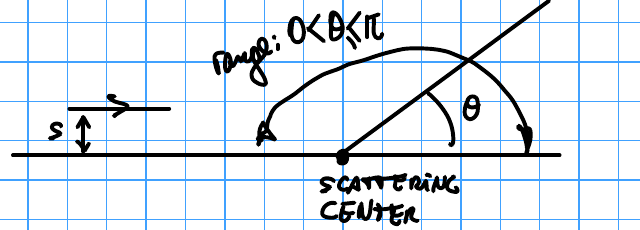
\includegraphics[width=0.62\textwidth]{scat_fig4_scattering_center.png}
\caption{Deflection about the scattering centre; the accessible range is
$0 < \theta \le \pi$.}
\label{fig:centre}
\end{figure}

\subsection*{Caveat}

\begin{enumerate}[label=\arabic*)]
\item In a dense conducting material:
\[
V = -\frac{k}{r}
\;\longrightarrow\;
V^{\textsc{screen}}(r) = -\frac{k}{r}\,e^{-r/\lambda}
\qquad
\begin{aligned}
&\text{screened Coulomb}\\
&\text{potential (``Yukawa'')}
\end{aligned}
\]
\end{enumerate}

\noindent(In non-conducting materials $V^{\textsc{screen}}(r)$ may take a different
form, but still will vanish much faster than $1/r$.)

\section*{Chapter 8 --- Hamiltonian and Hamilton's equations of motion}

\begin{center}
\fbox{\begin{minipage}{0.62\textwidth}
\centering
\textbf{MIDTERM REMARK}\\[3pt]
In polar coordinates
\[
\pd{L}{\dot\theta} = p_{\theta} = \ell_{z}
\]
\retracted{$L = L(r,\dot r, p_{\theta})$}\\[2pt]
\retracted{$\Downarrow$\quad Lagrange Eqn}\\[4pt]
{\scriptsize[the two lines above are struck out by a large red X in the original]}
\end{minipage}}
\end{center}

\[
L = T - V = L(q_{1}\ldots q_{n},\,\dot q_{1}\ldots \dot q_{n},\, t)
\]
\[
0 = \ddt{}\left(\evalat{\pd{L}{\dot q_{i}}}{\dot q_{j},\,q_{j}}\right)
  - \evalat{\pd{L}{q_{i}}}{\dot q_{j},\,q_{j}},
\qquad
p_{i} = \evalat{\pd{L}{\dot q_{i}}}{\dot q_{j},\,q_{j}} .
\]

\subsection*{Legendre transformation}

\[
q_{1}\ldots q_{n},\ \dot q_{1}\ldots \dot q_{n}
\;\longrightarrow\;
q_{1}\ldots q_{n},\ p_{1}\ldots p_{n}
\]
\[
f(x,y) \;\Longrightarrow\;
\d f = \pd{f}{x}\,\d x + \pd{f}{y}\,\d y .
\]

\subsubsection*{In thermodynamics}

\[
\text{1st Law}\qquad
\overset{\text{\scriptsize[fluid at constant $N$]}}{\d U = \,\dbar Q + \,\dbar W = T\,\d S - p\,\d V},
\qquad
U = U(S,V)\ \ \text{internal energy}
\]

We want $T,V$ as variables.
\[
F = A = U - TS \qquad \text{Helmholtz free energy}
\]
\[
\d A = \d U - \d(TS)
 = \cancel{T\,\d S} - p\,\d V - \cancel{T\,\d S} - S\,\d T
 = -S\,\d T - p\,\d V
\;\Longrightarrow\; A = A(T,V).
\]

\subsubsection*{In general}

The line below is written in the source with $f(x,y)$ on the left-hand side where
$\d f$ is meant.\footnote{Source reads ``In general $f(x,y) = u\,\d x + v\,\d y$'';
the left-hand side should be $\d f$, as the same page writes correctly two lines
above ($f(x,y) \Rightarrow \d f = \pd{f}{x}\d x + \pd{f}{y}\d y$) and uses correctly
one line below ($g = f - ux \Rightarrow \d g = \d f - \d(ux)$). Reproduced as written.}
\[
f(x,y) = u\,\d x + v\,\d y,
\qquad
u = \pd{f}{x},\qquad v = \pd{f}{y},
\qquad (x,y) \longrightarrow (u,y)
\]
\[
g = f - ux \;\Longrightarrow\;
\d g = \d f - \d(ux)
 = \cancel{u\,\d x} + v\,\d y - \cancel{u\,\d x} - x\,\d u
 = -x\,\d u + v\,\d y,
\qquad g = g(u,y).
\]

\subsection*{The Hamiltonian}

Let us look at $L(q_{1}\ldots q_{n},\,\dot q_{1}\ldots \dot q_{n})$, with
\[
\ovalbox{$\displaystyle p_{i} = \evalat{\pd{L}{\dot q_{i}}}{\dot q_{j},\,q_{j}}$}
\]
\[
H = -\left(L - \sum_{i} p_{i}\dot q_{i}\right)
\]
\begin{align*}
\d H &= -\d L + \sum_{i} \d\bigl(p_{i}\dot q_{i}\bigr)\\
     &= -\sum_{i}\left(\pd{L}{q_{i}}\,\d q_{i}
        + \cancel{\pd{L}{\dot q_{i}}\,\d\dot q_{i}}\right)
        \;-\;\pd{L}{t}\;
        +\;\sum_{i}\left(\cancel{p_{i}\,\d\dot q_{i}} + \dot q_{i}\,\d p_{i}\right)
\end{align*}
so that\footnote{The term $-\pd{L}{t}$ is inserted interlinearly in the source and
carries no $\d t$; the same omission is repeated in the line below, where the first
term of $\d H$ is written $-\pd{L}{t}$ rather than $-\pd{L}{t}\,\d t$. Reproduced as
written.}
\[
\d H = -\pd{L}{t} + \sum_{i}\left(\dot q_{i}\,\d p_{i}
  - \pd{L}{q_{i}}\,\d q_{i}\right)
\;\Longrightarrow\;
H = H(p_{1}\ldots p_{n},\, q_{1}\ldots q_{n},\, t).
\]

\begin{center}
\fbox{\begin{minipage}{0.9\textwidth}
\[
\pd{H}{p_{i}} = \dot q_{i},
\qquad
\pd{H}{q_{i}} = -\pd{L}{q_{i}}
  \overset{\text{\scriptsize Lagrange Eqn}}{=} -\dot p_{i},
\qquad
\pd{H}{t} = -\pd{L}{t} .
\]
\end{minipage}}\\[3pt]
\textsc{canonical eqs.\ of motion}
\end{center}

\end{document}
